% En esta seccion se presentan experimentos concretos efectuados, exitosos o fallidos, mediante figuras y capturas de pantalla debidamente tituladas y referenciadas en el cuerpo del reporte.
\section{Experimentos}

\subsection{Actividad 1: Creacion de una casa sencilla con OpenGL}
Empezamos probando la clase \texttt{House3D} con los mismos valores con los que ya veníamos trabajando en \texttt{Triangle3D}, es decir, \texttt{size = 0.5f}, usando el constructor de un solo parámetro (el que fija la altura del techo igual a \texttt{size}). Al compilar y correr el programa, la casa aparecía en pantalla, pero el techo se veía demasiado alto y puntiagudo en proporción al cuerpo del cubo, casi como una torre.

Para corregir esto probamos distintos valores de \texttt{roofHeight} llamando al constructor de dos parámetros. Terminamos usando \texttt{House3D(0.5f, 0.35f)}, que da una proporción de techo más parecida a una casa real, un poco menos alto que el ancho de la base; la comparación entre ambas proporciones se aprecia en la Figura \ref{fig:actividad1-casa}. También aprovechamos las teclas WASD y las flechas, que ya estaban implementadas en el proyecto, para mover la cámara y confirmar visualmente que la figura quedaba centrada en el origen sin importar desde qué ángulo la viéramos.

\begin{figure}[H]
    \centering
    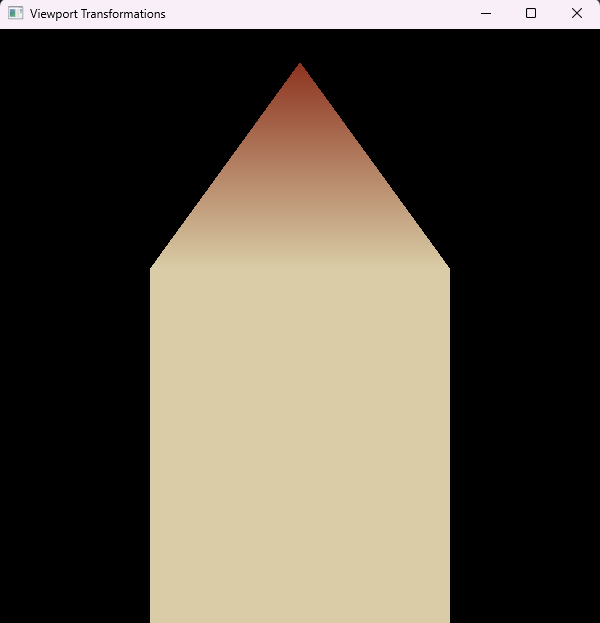
\includegraphics[width=0.45\textwidth]{Imagenes/E1/CasaPi.png}
    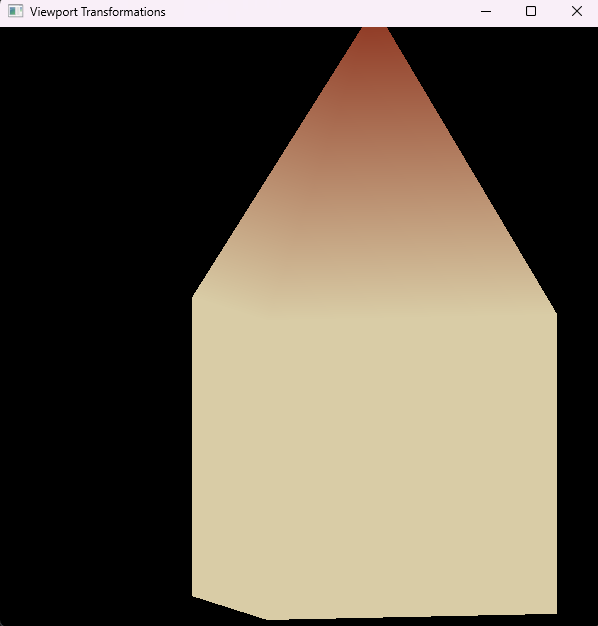
\includegraphics[width=0.45\textwidth]{Imagenes/E1/CasaPIO.png}
    \caption{Primeras pruebas de la casa: a la izquierda, el techo con la altura del constructor de un solo parámetro (\texttt{roofHeight = size}), que resultó demasiado puntiagudo; a la derecha, la misma figura tras ajustar la proporción.}
    \label{fig:actividad1-casa}
\end{figure}

Para verificar que la figura es realmente tridimensional y no un contorno
plano, giramos la cámara alrededor de ella con la proyección en perspectiva
activa. En la Figura \ref{fig:actividad1-perspectiva} se aprecian dos caras del
cubo al mismo tiempo y dos de las cuatro caras del techo, lo que confirma que
la construcción de los índices no dejó huecos entre las paredes.

\begin{figure}[H]
    \centering
    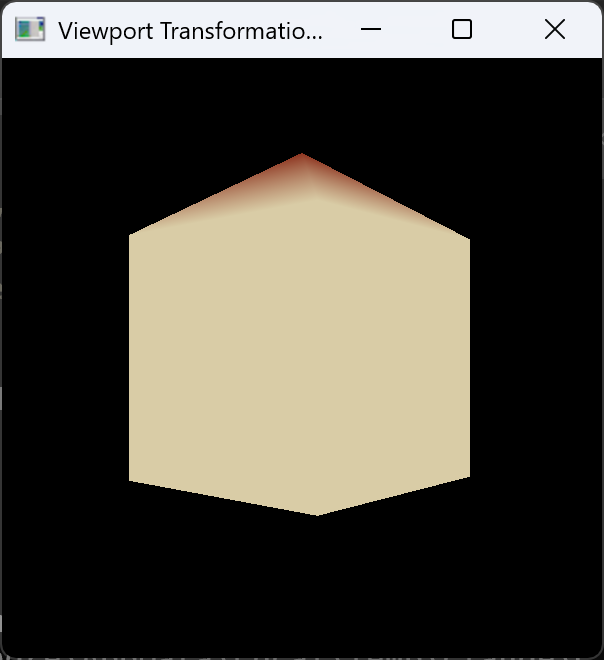
\includegraphics[width=0.5\textwidth]{Imagenes/E1/Casa_Perspectiva.png}
    \caption{La casa observada desde un ángulo intermedio con proyección en perspectiva.}
    \label{fig:actividad1-perspectiva}
\end{figure}


\subsection{Actividad 2: Configuración de las vistas: frontal, lateral y superior}
Para probar las vistas compilamos el proyecto y, con la ventana ya abierta, fuimos presionando F1, F2 y F3 mientras observábamos cómo cambiaba la casa en pantalla. Con la configuración original del código (antes de modificar los bloques de las teclas) notamos que F1 mostraba una vista en perspectiva diagonal, F2 mostraba la casa desde arriba y F3 la mostraba de frente; es decir, el orden no coincidía con lo que pedía la actividad (frontal, lateral y superior, en ese orden).

Después de reescribir los tres bloques con las posiciones sobre los ejes $X$, $Y$ y $Z$, volvimos a probar: F1 mostraba la fachada de la casa completamente de frente, con el techo apuntando hacia arriba de la pantalla; F2 mostraba el perfil lateral, dejando ver la silueta triangular del techo desde el costado; y F3 mostraba la vista de planta, con el contorno cuadrado de la base y el pico del techo justo en el centro, tal como se observa en la Figura \ref{fig:actividad2-vistas}. También probamos, a propósito, qué pasaba si dejábamos \texttt{Up = (0,1,0)} en la vista superior, y efectivamente la cámara perdía la orientación y la imagen se veía distorsionada, lo que confirmó que el ajuste del vector \texttt{Up} era necesario y no solo un detalle estético.

\begin{figure}[H]
    \centering
    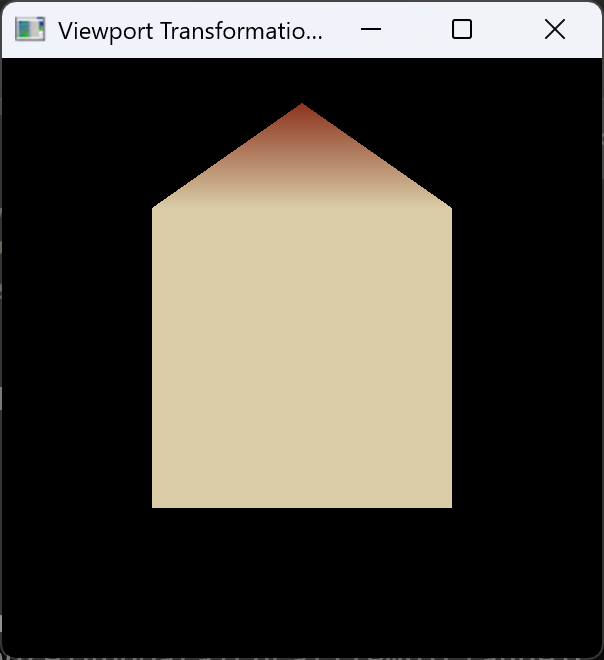
\includegraphics[width=0.32\textwidth]{Imagenes/E2/V_Frontal.png}
    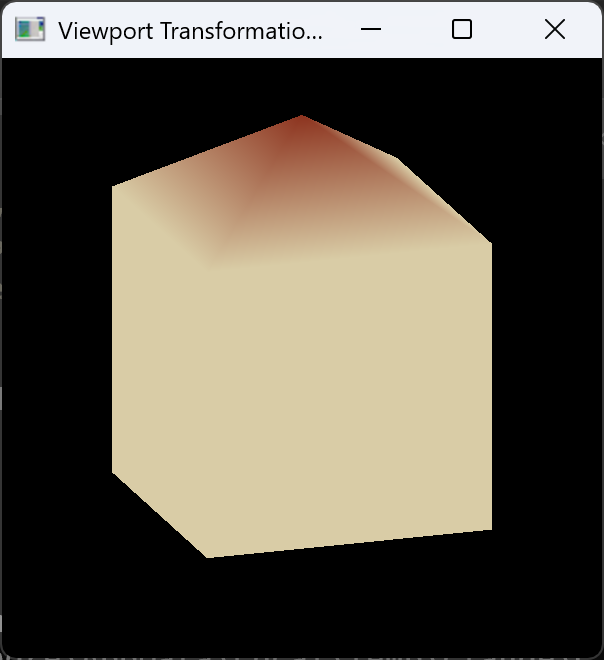
\includegraphics[width=0.32\textwidth]{Imagenes/E2/V_Lateral.png}
    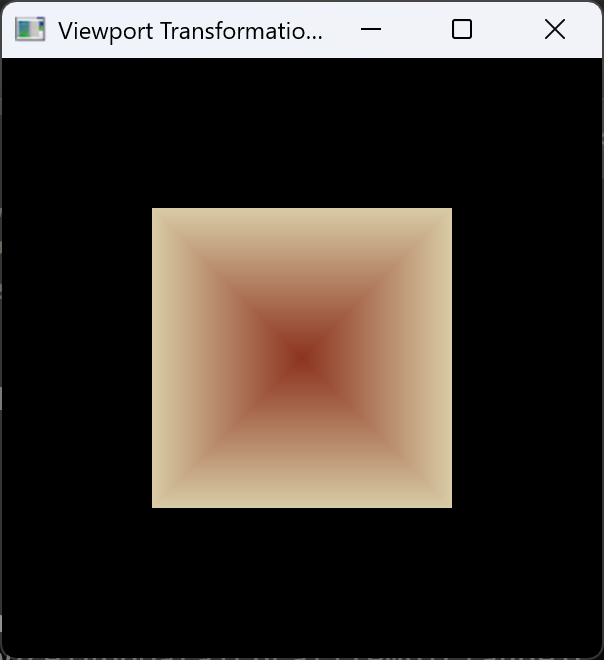
\includegraphics[width=0.32\textwidth]{Imagenes/E2/V_Superior.png}
    \caption{Pruebas de las tres vistas: frontal (\texttt{F1}), lateral (\texttt{F2}) y superior (\texttt{F3}).}
    \label{fig:actividad2-vistas}
\end{figure}

\subsection{Actividad 3: 3 vistas de proyección ortogonal}
El experimento consistió en dejar la cámara inmóvil en la vista frontal y
cambiar únicamente los argumentos de \texttt{glm::ortho} con las teclas
\texttt{1}, \texttt{2} y \texttt{3}, de modo que cualquier diferencia en la
imagen fuera atribuible sólo a la matriz de proyección. Los tres resultados se
muestran en la Figura \ref{fig:actividad3-experimentos}.

Con el volumen unitario, que es el del código original, la casa ocupa
aproximadamente la mitad de la ventana. Al duplicar los cuatro límites
laterales, la figura se redujo justo a la mitad de su tamaño anterior: el
volumen de visualización abarca el doble en cada dirección y, como se sigue
proyectando sobre la misma ventana, todo se dibuja a la mitad de escala. Este
resultado nos sirvió para descartar la idea intuitiva de que ampliar los
argumentos «acerca» la cámara; lo que hace es lo contrario.

La tercera variante fue la más reveladora. Al abrir sólo el intervalo
horizontal a $[-2,2]$ y dejar el vertical en $[-1,1]$, la casa apareció
comprimida: conserva su altura pero pierde la mitad de su ancho. La razón es
que el volumen dejó de ser proporcional a la ventana, que es cuadrada, así que
las unidades del mundo ya no miden lo mismo en $x$ que en $y$. La primera vez
que vimos esta imagen pensamos que habíamos alterado la geometría por error, y
sólo al volver a la variante uno y comprobar que la casa recuperaba su forma
confirmamos que el problema estaba en la proyección y no en los vértices.

\begin{figure}[H]
    \centering
    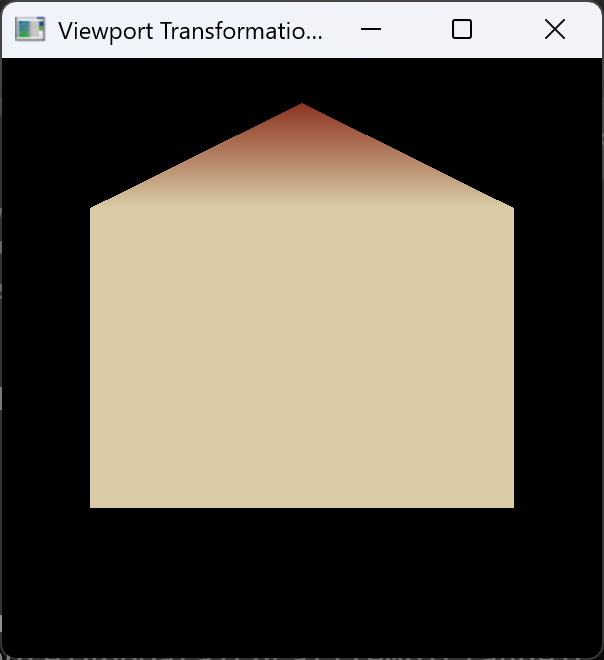
\includegraphics[width=0.32\textwidth]{Imagenes/E3/Ortho_Unitario.png}
    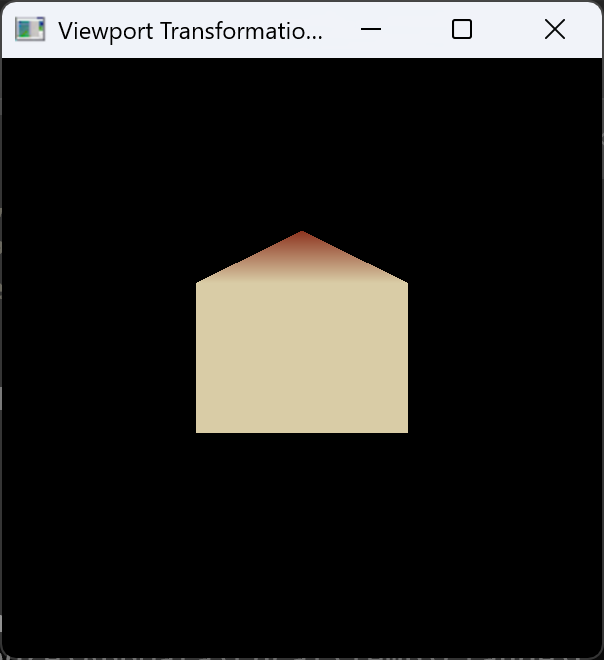
\includegraphics[width=0.32\textwidth]{Imagenes/E3/Ortho_Ampliado.png}
    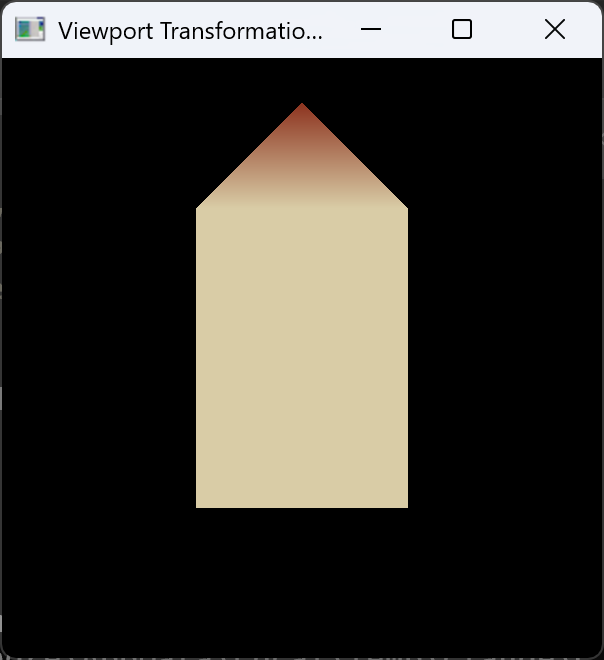
\includegraphics[width=0.32\textwidth]{Imagenes/E3/Ortho_Anisotropo.png}
    \caption{Las tres variantes de proyección ortogonal, con la cámara fija: volumen unitario (izquierda), volumen ampliado al doble (centro) y volumen anisótropo, más ancho que alto (derecha).}
    \label{fig:actividad3-experimentos}
\end{figure}

\subsection{Actividad 4: 3 vistas de proyección perspectiva}
Repetimos el mismo procedimiento con la proyección en perspectiva: cámara
inmóvil en la vista frontal y cambio del ángulo de apertura con las teclas
\texttt{4}, \texttt{5} y \texttt{6}. Lo primero que notamos, ya al pasar de la
proyección ortogonal a la de perspectiva, fue la aparición del escorzo: la
pared frontal se dibuja más grande que la trasera y las aristas del techo dejan
de ser paralelas en la imagen, algo que no ocurría en ninguna de las variantes
de la actividad anterior.

Con $90^\circ$ el efecto se exagera. La casa se reduce de manera notable porque
el frustum abarca mucho más escena, y la deformación cerca de los bordes de la
ventana se hace evidente. Con $30^\circ$ ocurrió lo contrario y de paso
obtuvimos un resultado que, en un primer intento, dimos por fallido: la casa
creció tanto que el vértice del techo quedó recortado por el borde superior de
la ventana. Al revisarlo entendimos que no se trataba de un error de
programación, sino del comportamiento esperado, ya que un frustum tan estrecho
deja fuera de la escena todo lo que no cabe en el ángulo de apertura. Además,
en esa variante el escorzo casi desaparece y la imagen se parece a la de la
proyección ortogonal, lo que ilustra bien que la proyección ortogonal puede
verse como el caso límite de la perspectiva cuando el observador se aleja
indefinidamente.

\begin{figure}[H]
    \centering
    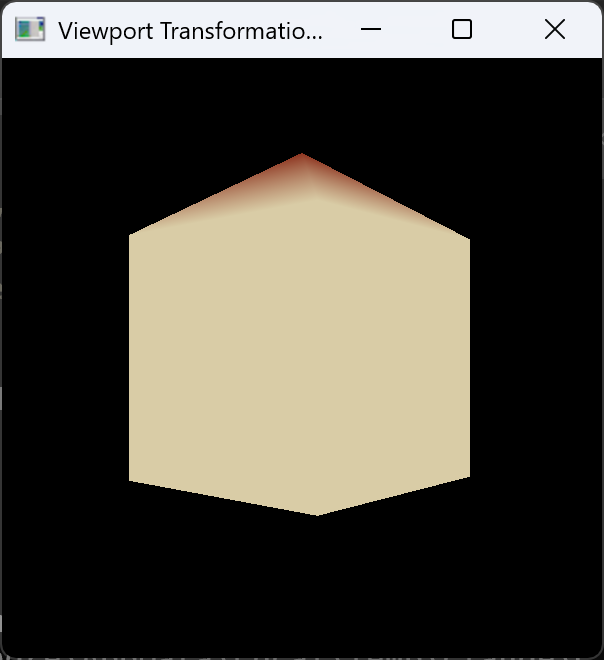
\includegraphics[width=0.32\textwidth]{Imagenes/E4/Persp_45.png}
    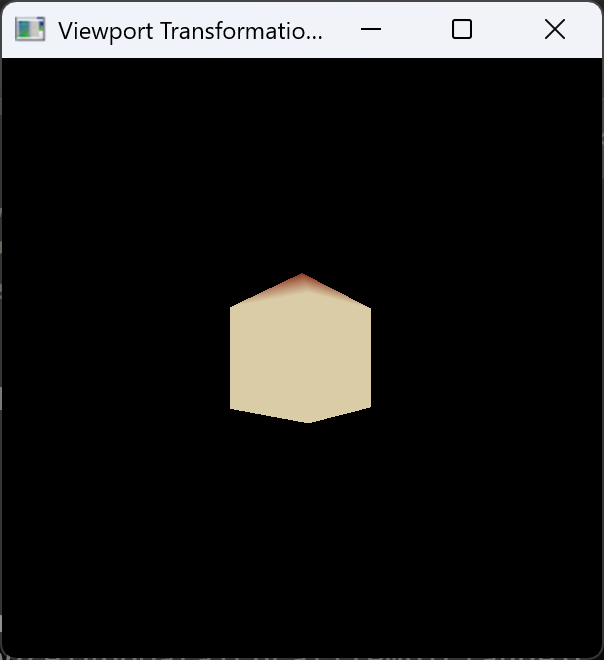
\includegraphics[width=0.32\textwidth]{Imagenes/E4/Persp_90.png}
    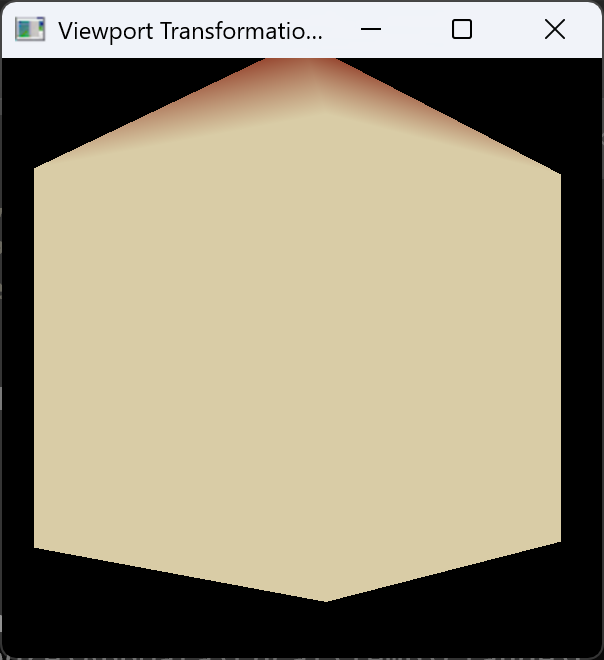
\includegraphics[width=0.32\textwidth]{Imagenes/E4/Persp_30.png}
    \caption{Las tres variantes de proyección en perspectiva, con la cámara fija: apertura de $45^\circ$ (izquierda), $90^\circ$ (centro) y $30^\circ$ (derecha). En esta última la figura se recorta contra el borde superior de la ventana.}
    \label{fig:actividad4-experimentos}
\end{figure}

\subsection{Actividad 5: Implementación de la camara usando WASD}
Probamos la cámara recorriendo la órbita y variando el radio hasta sus dos
extremos. En la Figura \ref{fig:actividad5-experimentos} se muestran los tres
casos: la casa vista desde otro ángulo, el acercamiento máximo y el alejamiento
máximo. En los tres, la figura permanece centrada en la ventana, que era la
conducta que buscábamos al describir la posición del observador con un ángulo y
un radio en lugar de coordenadas cartesianas.

\begin{figure}[H]
    \centering
    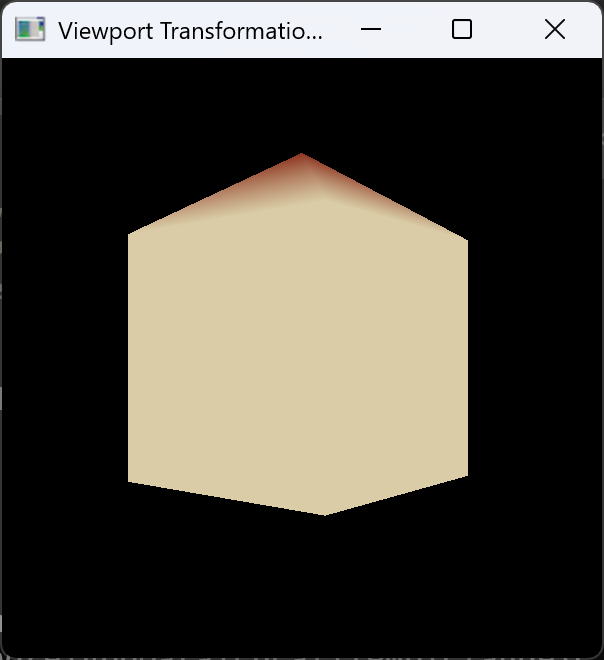
\includegraphics[width=0.32\textwidth]{Imagenes/E5/Cam_GiroA.png}
    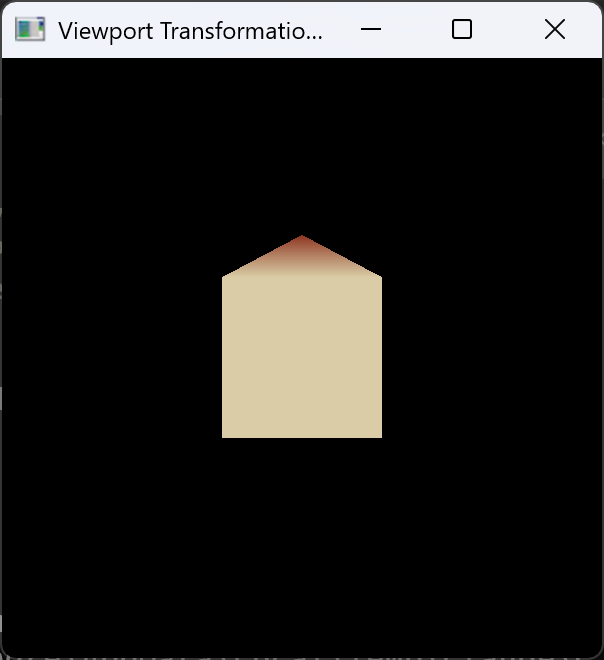
\includegraphics[width=0.32\textwidth]{Imagenes/E5/Cam_Lejos.png}
    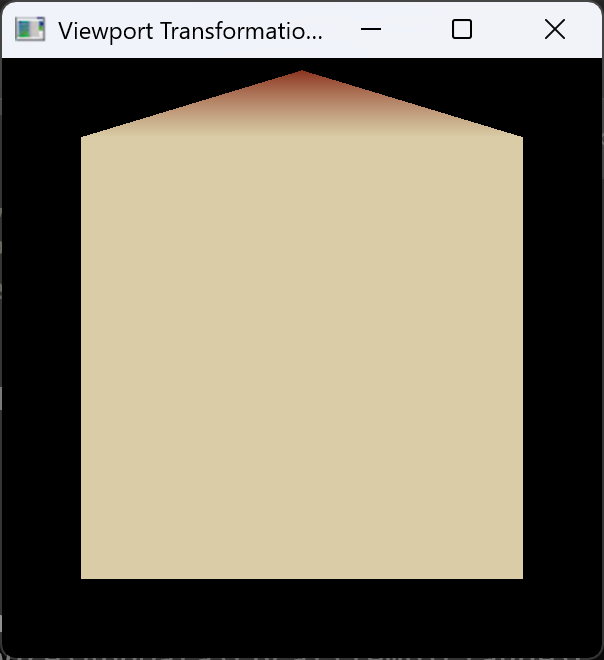
\includegraphics[width=0.32\textwidth]{Imagenes/E5/Cam_Cerca.png}
    \caption{Experimentos con la cámara: vista desde otro ángulo, alejamiento máximo y acercamiento máximo.}
    \label{fig:actividad5-experimentos}
\end{figure}

\subsection{Actividad 6: Implementación de las flechas del teclado con respecto al eje Z}

Para el experimento, primero probamos mover la casa dejando el valor de avance en $0.01\text{f}$ como venía en el código original. Al presionar las flechas arriba y abajo la figura sí se movía sobre el eje $Z$, pero iba bastante lento; teníamos que dejar la tecla aplastada mucho tiempo para notar que se alejaba o se acercaba. Además, si la mirábamos de frente casi no se notaba la profundidad, solo parecía como si la casa se hiciera chiquita o grandota.

Como variación, decidimos subirle el número del incremento a $0.05\text{f}$ para que el movimiento fuera más rápido y no tan pesado de probar. También cambiamos la cámara a la vista en diagonal usando la tecla F1, porque desde esa esquina inclinada sí se alcanza a ver claramente todo el recorrido de la casa en tres dimensiones hacia adelante y hacia atrás.

Al correr el programa con estos cambios, la figura respondió mucho mejor y fue mucho más fácil de controlar. La casa se desplazó de forma pareja por toda la pantalla sin trabarse ni perder su forma, con lo que pudimos comprobar que la traslación sobre el eje $Z$ funciona perfectamente bien.

\begin{lstlisting}[language=C++, caption={Variación de la velocidad de desplazamiento en el eje Z (keyboardCallback)}]
// Variación Actividad 6: Incremento ajustado a 0.05f para mayor fluidez
float stepZ = 0.05f;

// Flecha Arriba: avanzar en +Z
if (glfwGetKey(window, GLFW_KEY_UP) == GLFW_PRESS) {
    modelPosition.Position.z += stepZ;
}

// Flecha Abajo: retroceder en -Z
if (glfwGetKey(window, GLFW_KEY_DOWN) == GLFW_PRESS) {
    modelPosition.Position.z -= stepZ;
}
\end{lstlisting}

La primera prueba la hicimos desde la vista frontal, que es la que teníamos
activa mientras programábamos, y estuvo a punto de hacernos pensar que la
traslación no funcionaba: la casa no se movía de lugar, únicamente cambiaba de
tamaño. Tardamos un momento en caer en la cuenta de que ése es exactamente el
resultado correcto, porque desde el eje $+Z$ la cámara mira a lo largo de la
misma dirección en la que se desplaza el modelo, de modo que el movimiento se
proyecta sobre un punto y lo único que percibimos es el escorzo. La Figura
\ref{fig:actividad6-frontal} muestra las tres posiciones.

\begin{figure}[H]
    \centering
    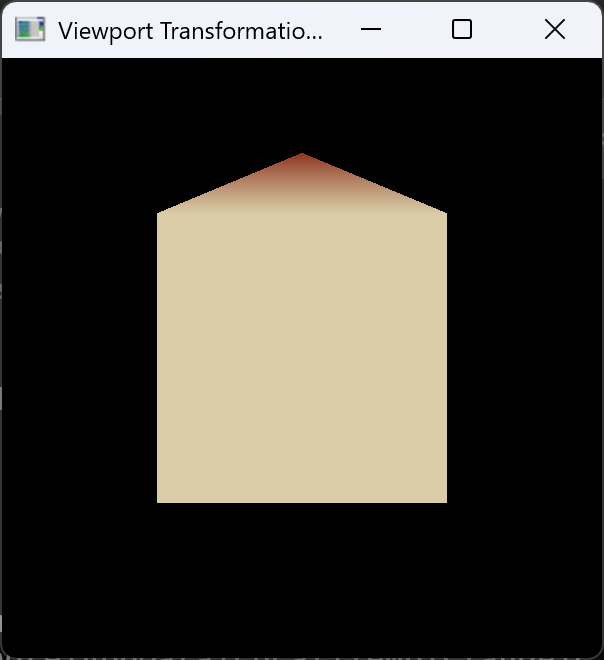
\includegraphics[width=0.32\textwidth]{Imagenes/E6/Z_Inicial.png}
    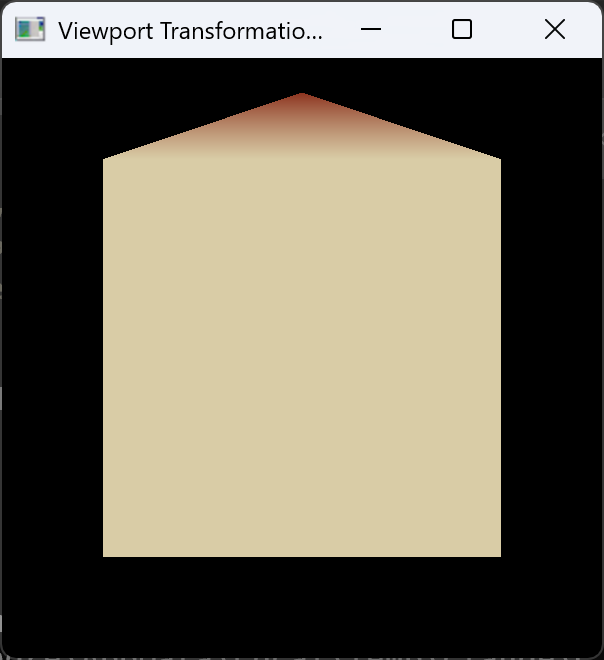
\includegraphics[width=0.32\textwidth]{Imagenes/E6/Z_Avance.png}
    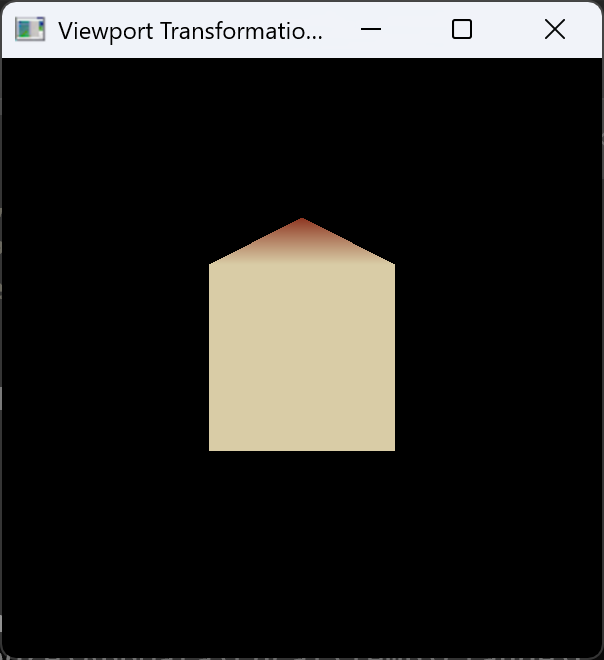
\includegraphics[width=0.32\textwidth]{Imagenes/E6/Z_Retroceso.png}
    \caption{Traslación sobre el eje $Z$ vista desde el frente: posición inicial (izquierda), avance con la flecha arriba (centro) y retroceso con la flecha abajo (derecha).}
    \label{fig:actividad6-frontal}
\end{figure}

Para comprobarlo repetimos el experimento desde la vista lateral, presionando
\texttt{F2} antes de mover el modelo. Ahí el desplazamiento se ve directamente
como lo que es: la casa recorre la escena de un lado a otro de la ventana sin
cambiar de tamaño de forma apreciable, tal como se observa en la Figura
\ref{fig:actividad6-lateral}. Esta pareja de pruebas fue la más útil de toda la
práctica, porque muestra que una misma transformación puede producir efectos
visuales completamente distintos según desde dónde se le observe.

\begin{figure}[H]
    \centering
    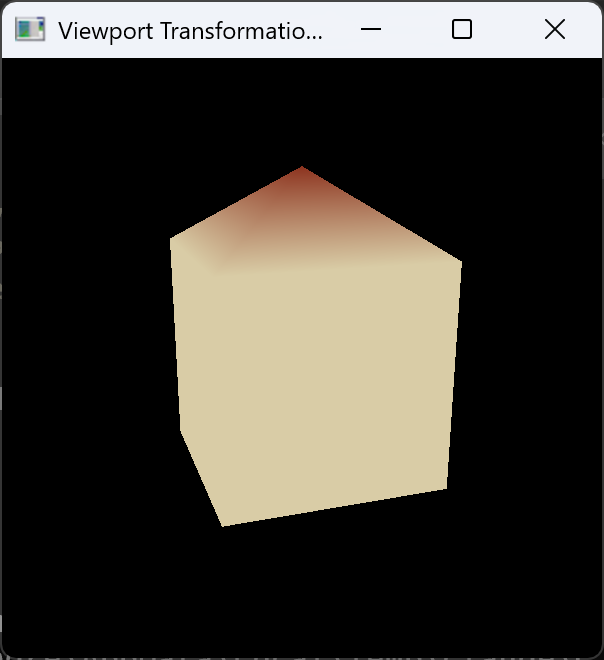
\includegraphics[width=0.32\textwidth]{Imagenes/E6/Z_Lat_Inicial.png}
    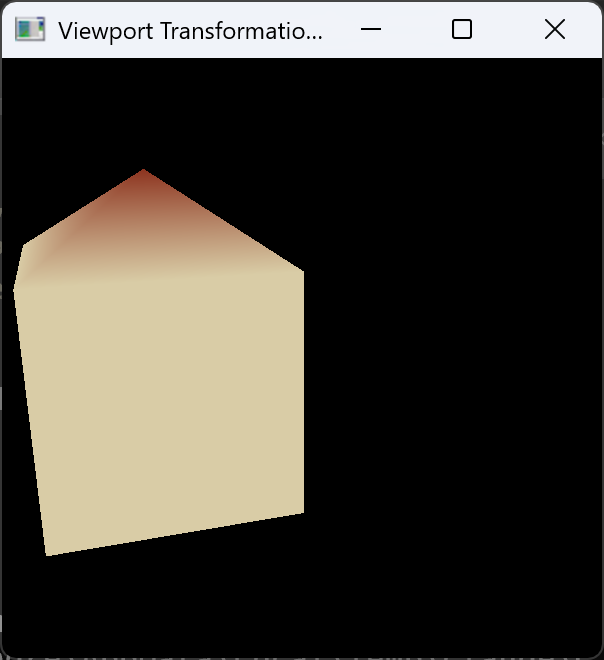
\includegraphics[width=0.32\textwidth]{Imagenes/E6/Z_Lat_Avance.png}
    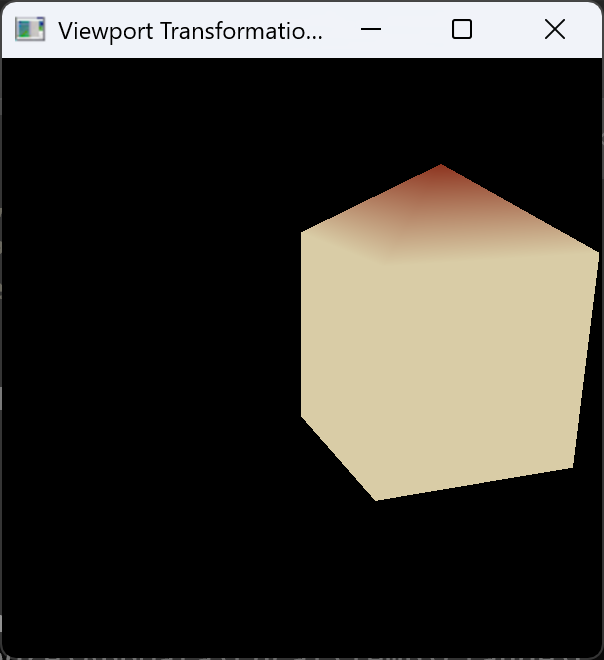
\includegraphics[width=0.32\textwidth]{Imagenes/E6/Z_Lat_Retroceso.png}
    \caption{La misma traslación sobre el eje $Z$ observada desde la vista lateral: posición inicial (izquierda), avance (centro) y retroceso (derecha).}
    \label{fig:actividad6-lateral}
\end{figure}

Como tercera variación cambiamos la proyección a ortogonal y volvimos a mover
la casa desde la vista frontal. El resultado, que se muestra en la Figura
\ref{fig:actividad6-ortho}, es que la figura no cambia en absoluto: las dos
capturas son idénticas aunque entre una y otra el modelo se desplazó varias
unidades sobre el eje $Z$. Esto confirma que en la proyección ortogonal la
distancia al observador no interviene en el tamaño de la imagen, y que el
cambio de tamaño que habíamos visto antes provenía de la división por la
componente homogénea de la proyección en perspectiva y no de la traslación.

\begin{figure}[H]
    \centering
    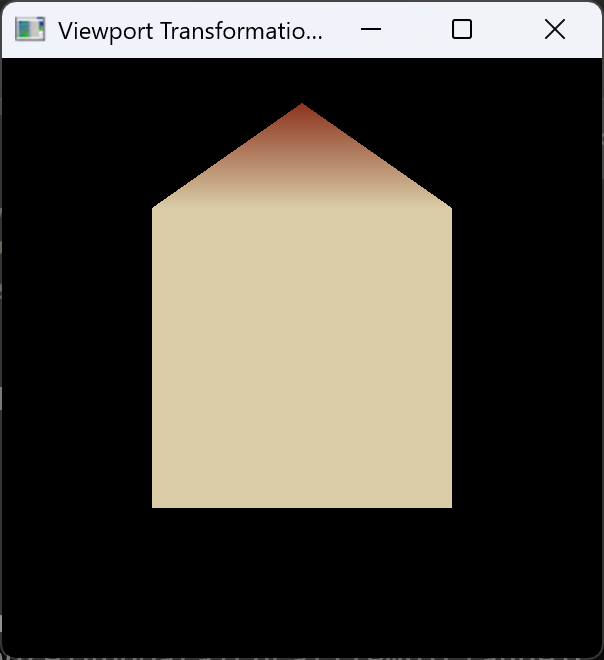
\includegraphics[width=0.4\textwidth]{Imagenes/E6/Z_Ortho_Inicial.png}
    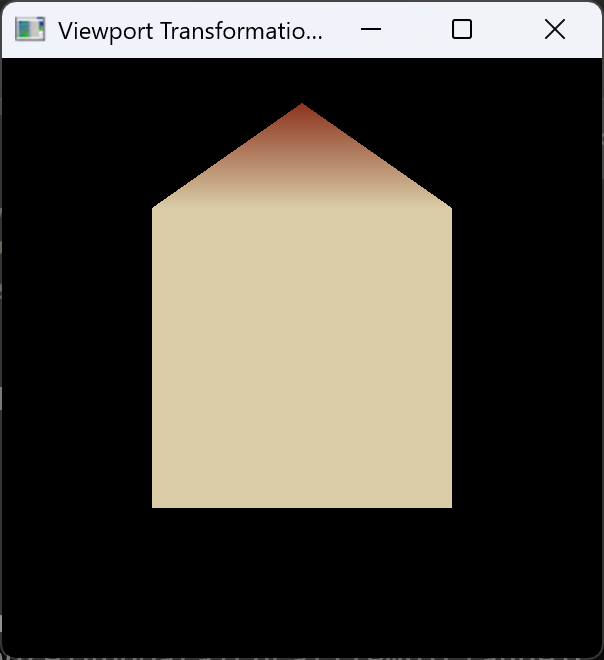
\includegraphics[width=0.4\textwidth]{Imagenes/E6/Z_Ortho_Avance.png}
    \caption{Traslación sobre el eje $Z$ con proyección ortogonal: antes (izquierda) y después (derecha) de desplazar el modelo. La imagen no cambia.}
    \label{fig:actividad6-ortho}
\end{figure}

\subsection{Actividad 7: Implementación de las teclas + y - para aumentar y disminuir el tamaño de la geometría}
El primer intento de esta actividad no funcionó y la causa nos costó
encontrarla. Habíamos asignado el escalamiento a \texttt{GLFW\_KEY\_KP\_ADD} y
\texttt{GLFW\_KEY\_KP\_SUBTRACT}, que son las teclas del teclado numérico, tal
como aparecen en el código base; al probarlo en una computadora portátil sin
teclado numérico las teclas simplemente no respondían, y estuvimos revisando la
matriz de modelo buscando un error que no existía. La solución fue aceptar
también \texttt{GLFW\_KEY\_EQUAL} y \texttt{GLFW\_KEY\_MINUS}, del bloque
alfanumérico.

Una vez resuelto eso, el experimento consistió en llevar el factor de escala
por encima y por debajo de la unidad partiendo de la vista frontal. Para que
los tres tamaños cupieran en la misma ventana usamos la variante ampliada de la
proyección ortogonal, ya que con el volumen unitario la casa agrandada se salía
del encuadre. Los resultados se muestran en la Figura
\ref{fig:actividad7-experimentos}: la casa crece y se reduce manteniendo sus
proporciones y, sobre todo, sin desplazarse del centro de la ventana, que era
la conducta que buscábamos.

También probamos, a propósito, qué ocurría al quitar los límites del factor de
escala. Al mantener presionada la tecla \texttt{-} el valor cruzó el cero y se
volvió negativo, con lo que la casa se invirtió y el techo apareció por debajo
del piso, mientras que al mantener \texttt{+} la geometría terminó atravesando
el plano cercano del volumen de visualización y la ventana se llenó por
completo. Ambos casos nos convencieron de dejar las cotas de $0.05$ y $5.0$ en
la versión final.

\begin{figure}[H]
    \centering
    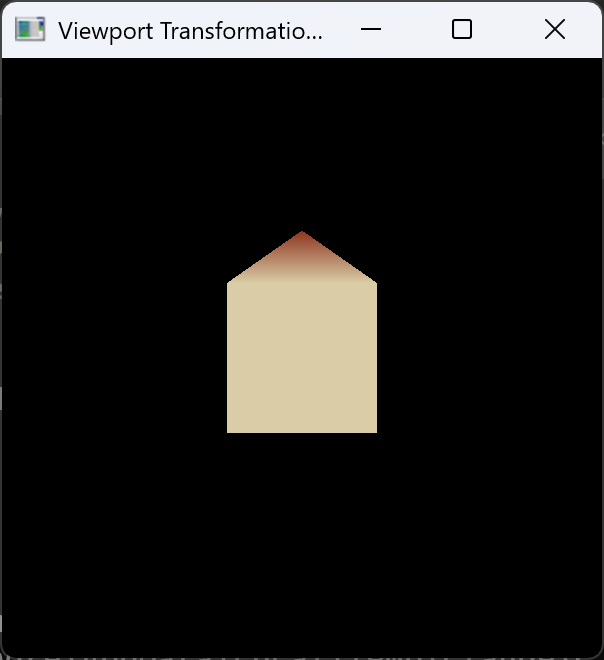
\includegraphics[width=0.32\textwidth]{Imagenes/E7/Escala_Inicial.png}
    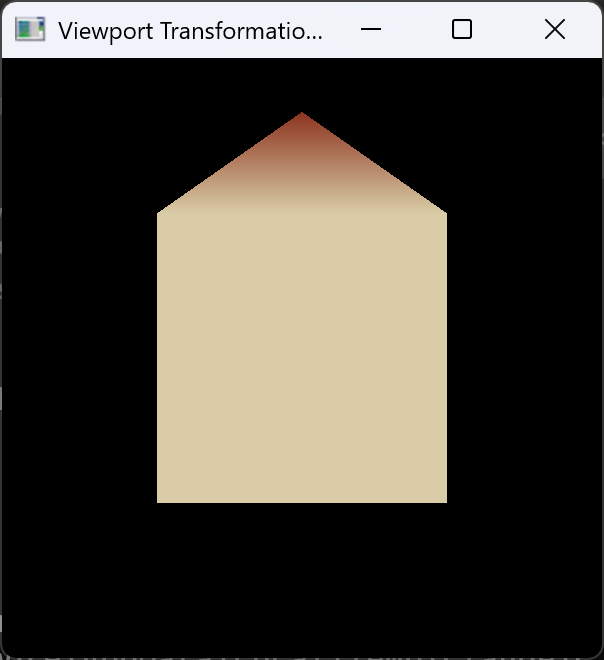
\includegraphics[width=0.32\textwidth]{Imagenes/E7/Escala_Mayor.png}
    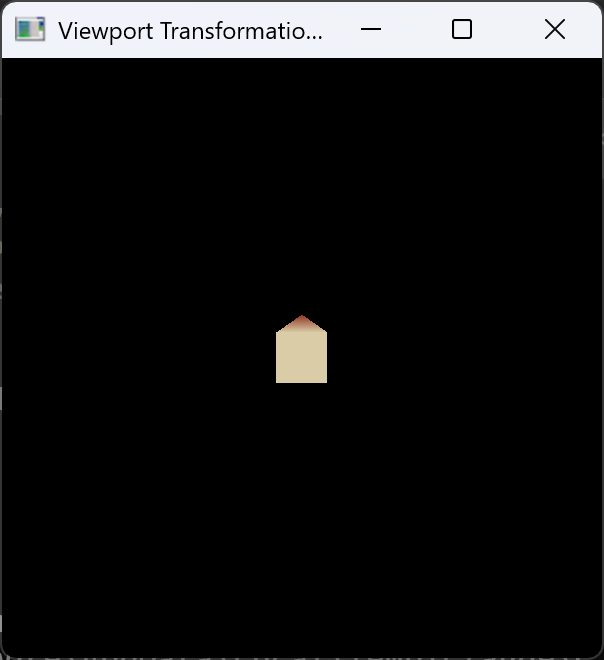
\includegraphics[width=0.32\textwidth]{Imagenes/E7/Escala_Menor.png}
    \caption{Escalamiento uniforme del modelo: factor unitario (izquierda), aumento con la tecla \texttt{+} (centro) y reducción con la tecla \texttt{-} (derecha).}
    \label{fig:actividad7-experimentos}
\end{figure}